\section{Ausblick}

Nachdem nun die aktuelle Situation des heutigen Internets aufgezeigt und die möglichen Entwicklungen in der Zukunft erläutert wurden, soll das letzte Kapitel sich damit beschäftigen, inwieweit die Dezentralisierung im Bezug auf das Internet Einzug finden kann beziehungsweise wird.

\begin{figure*}
	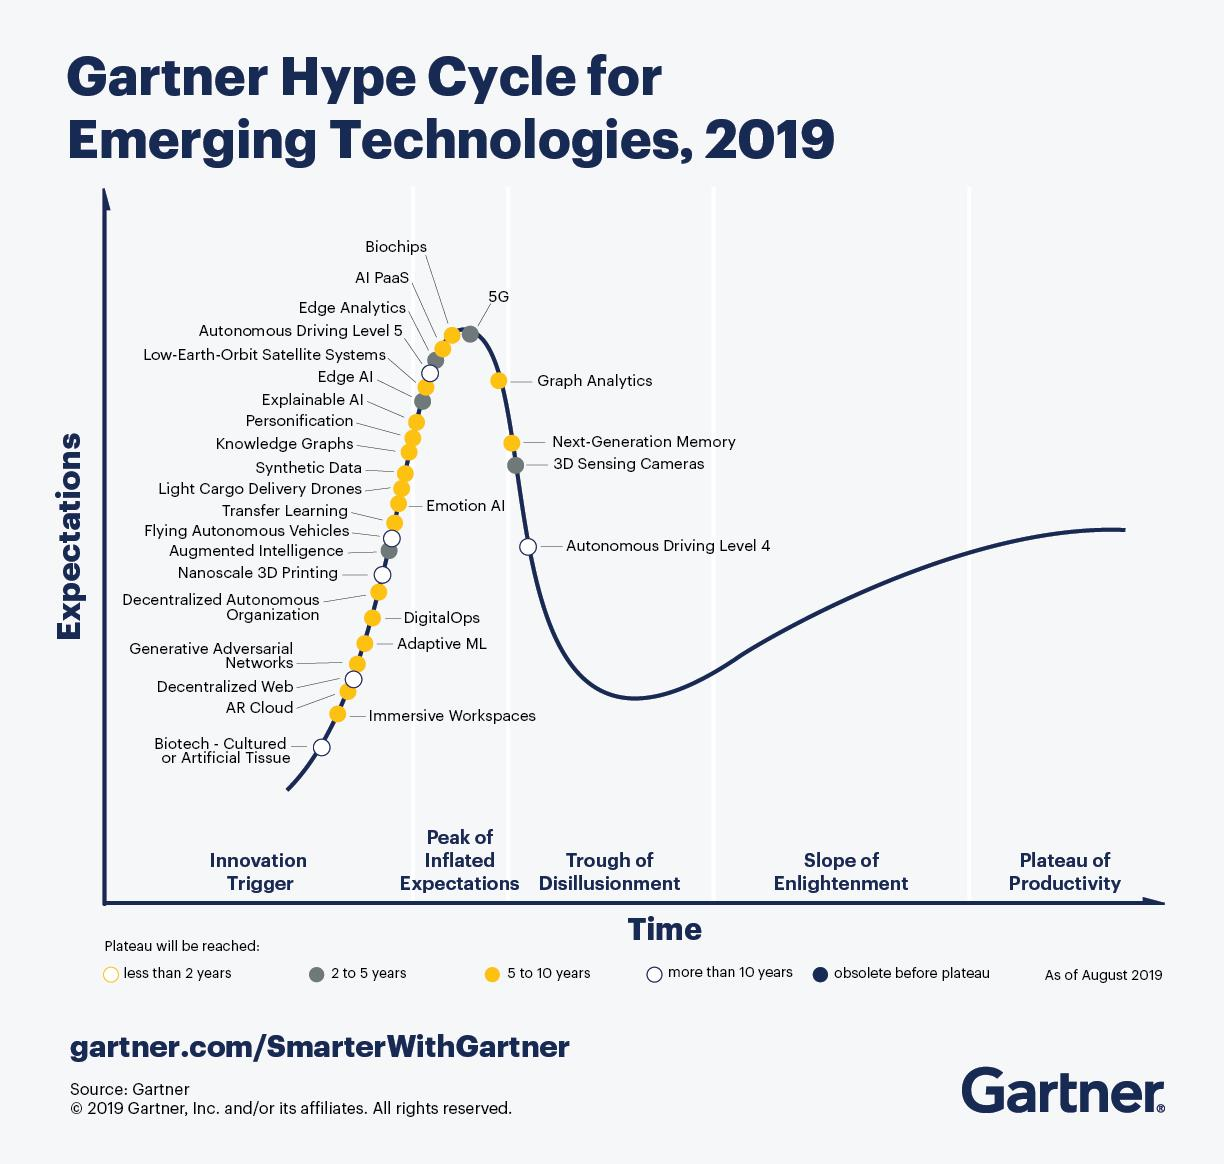
\includegraphics[width=\linewidth]{images/5TrendsAppear.jpg}
	\caption{Gartner Hype Cycle for Emerging Technologies, 2019~\cite{Panetta.2019}}
	\label{fig:gartnerhype}
\end{figure*}

Wie in Figure~\ref{fig:gartnerhype} zu sehen, befindet sich die Technologie \textit{Decentralized Web} noch ziemlich am Anfang des Gartner Hype Cycle's, und der Zeitraum bis zur Etablierung ist auf 10 Jahre geschätzt. 
Wie bereits angesprochen, sieht man immer mehr Unternehmen, Organisationen und damit letztlich Menschen an der Technologie arbeiten. Dies liegt hauptsächlich daran, dass es die heutigen Tech-Konzerne mit der Verletzung der Privatsphäre zu weit getrieben haben. Letztendlich arbeiten viele Personen freiwillig an der Technologie, weil sie für ein freies Internet kämpfen, in dem die Nutzung von Diensten nicht mit seinen privaten Daten "'erkauft"' wird. Denn nichts anderes passiert in der jetzigen Zeit des Web2: Die frühen Anbieter von Services im Internet haben sehr schnell mitbekommen, dass Nutzer nicht bereit dafür sind, für die Nutzung der Dienste im Web zu bezahlen. Also suchten sie nach anderen Möglichkeiten, Profit zu generieren, und dadurch entwickelte sich die heutige Kommerzialisierung mit Nutzerdaten.


Und dieses Konzept war nie im Sinne des Erfinders. Der durch seine Pionier-Arbeit am World Wide Web zum Ritter geschlagene Sir Timothy Berners-Lee hat nie auch nur ansatzweise ein Vermögen mit seiner Erfindung verdient, er wollte lediglich das Leben der Menschen verbessern und vereinfachen. 
Nun arbeitet er schon länger am sogenannten Solid-Projekt~\cite{Clark.2018}. 
Die Abkürzung steht für Social Linked Data und zielt darauf ab, den großen Technik-Firmen die Nutzerdaten aus ihren Daten-Silos zu entziehen und diese in sogenannten Pods zu speichern, die der Nutzer selbst kontrolliert. 
So soll beispielsweise ein Umzug von Firma A zu Firma B problemlos möglich sein: Man entzieht A ganz einfach die Berechtigung auf den eigenen Datenpod und gewährt sie B~\cite{Park.2018}. 

\smallskip

Dies wird jedoch schwieriger, als auf den ersten Blick ersichtlich: Die Konzerne, gegen die das Projekt gerichtet ist, werden sich wohl kaum an einer einheitlichen Lösung beteiligen, und für neue oder kleine Firmen fehlt es an Nutzerzahlen und damit an Investoren~\cite{Park.2018}. Dieses Problem entstand laut Steven Johnson, weil die von ihm als "'InternetOne"' bezeichnete Schicht offene Protokolle wie TCP/IP und HTML verwendeten, und die Verwaltung von Identitäten und persönlichen Daten auf das "'InternetTwo"' ausgelagert wurden. Die Protokolle dieser zweiten Schicht wurden jedoch vornehmlich von Unternehmen definiert, weshalb kaum Standards im Bereich der Datensicherheit existieren~\cite{Bonset.2019}. 

\smallskip

All das Engagement zeigt, dass vor allem das Thema der Privatsphäre und des gläsernen Bürgers in den Vordergrund rückt. Doch eine schnelle Änderung der Situation wird dies wohl nicht bewirken, dafür verzeichnen die etablierten Plattformen zu große Nutzerzahlen, und es gibt noch zu wenige beziehungsweise keine konkurrenzfähigen Alternativen.

Vermutlich werden in der Zukunft Unternehmen die Technologie der Dezentralisierung weiter vorantreiben und auch einsetzen, bevor diese vollumfänglich in den privaten Sektor vordringt. Denn durch die Blockchain stehen vor allem Unternehmen enorm viele Möglichkeiten offen, da diese nicht nur Prozesse vereinfachen und automatisieren kann, sondern auch hohe Kostensenkungen ermöglicht.

Fakt ist, dass die Technologie noch viele Jahre zur Marktreife benötigt. Nichtsdestotrotz stellt sie jedoch eine realistische Alternative zum Marktmonopol einiger weniger Unternehmen dar, und diese Alternative wird mit zunehmenden Jahren immer dringender benötigt. Die Veränderung zum dezentralen Web wird jedoch nach und nach Anklang finden, je nachdem wie die Entwicklung voranschreitet und die Technik in der Gesellschaft angenommen wird.





